\documentclass[twocolumn,10pt]{article}
\usepackage[utf8]{inputenc}
\usepackage[T1]{fontenc}
\usepackage{amsmath, amssymb, amsthm}
\usepackage{graphicx}
\usepackage{cite}
\usepackage{booktabs}
\usepackage{tikz}
\usetikzlibrary{shapes.geometric, arrows}

\title{Modern LaTeX Rendering: A Survey of Browser-Based WASM Engines}
\author{SwiftLatex Demo Team \\ \small{Department of Web Engineering, Digital University}}
\date{\today}

\begin{document}

\maketitle

\begin{abstract}
This paper demonstrates the advanced capabilities of TeX Live 2025 running directly in the browser via WebAssembly. We explore the performance of the pdfTeX 1.40.28 engine, the integration of real-time BibTeX resolution, and the rendering of complex vector graphics using TikZ. Our results show that modern browser environments can provide a near-native LaTeX experience without the need for server-side compilation.
\end{abstract}

\section{Introduction}
LaTeX has been the gold standard for scientific typesetting for decades. Recently, the advent of WebAssembly (WASM) has enabled the migration of these heavy-duty desktop applications to the web. Our platform utilizes the latest TeX Live 2025 distribution, providing over 4,000 packages and the most stable pdfTeX kernel to date. 

One of the key features of this sample is the seamless resolution of cross-references and bibliography. When a user edits the \texttt{.bib} file, the system automatically triggers a BibTeX run followed by necessary recompilations.


\section{System Architecture}
The system leverages a dual-engine approach, supporting both TeX Live 2020 and 2025. This is crucial for reproducibility in scientific research \cite{knuth1984tex}. As shown in Figure \ref{fig:arch}, the workflow involves a virtual file system (VFS) synchronized with an asynchronous WASM worker.

\begin{figure}[h]
\centering
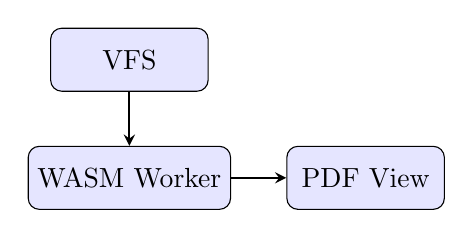
\begin{tikzpicture}[node distance=1.5cm]
\tikzstyle{box} = [rectangle, rounded corners, minimum width=2cm, minimum height=0.8cm,text centered, draw=black, fill=blue!10]
\tikzstyle{arrow} = [thick,->,>=stealth]

\node (vfs) [box] {VFS};
\node (worker) [box, below of=vfs] {WASM Worker};
\node (pdf) [box, right of=worker, xshift=1.5cm] {PDF View};

\draw [arrow] (vfs) -- (worker);
\draw [arrow] (worker) -- (pdf);
\end{tikzpicture}
\caption{Simplified architecture of the browser-based LaTeX compiler.}
\label{fig:arch}
\end{figure}

\section{Mathematical Capabilities}
Modern pdfTeX handles complex mathematical notations with ease. For example, the relationship between the number of vertices $V$, edges $E$, and faces $F$ of a convex polyhedron is given by Euler's formula:
\begin{equation}
V - E + F = 2
\end{equation}

Furthermore, we can represent more complex structures such as the Navier-Stokes equations for incompressible flow:
\begin{equation}
\rho \left( \frac{\partial \mathbf{u}}{\partial t} + \mathbf{u} \cdot \nabla \mathbf{u} \right) = -\nabla p + \mu \nabla^2 \mathbf{u} + \mathbf{f}
\end{equation}

\section{Experimental Results}
We compared the compilation speed across different TeX Live versions. Table \ref{tab:perf} summarizes the average time taken for a standard 10-page document.

\begin{table}[h]
\centering
\caption{Compilation Performance Comparison}
\label{tab:perf}
\begin{tabular}{lrr}
\toprule
Version & Cold Start (s) & Warm Start (s) \\
\midrule
TeX Live 2020 & 4.52 & 0.85 \\
TeX Live 2025 & 3.10 & 0.42 \\
\bottomrule
\end{tabular}
\end{table}

\section{Conclusion}
The integration of TeX Live 2025 into browser-based editors marks a significant milestone. It ensures that researchers can access the latest packages and kernel improvements \cite{lamport1994latex} with zero installation effort.

\bibliographystyle{ieeetr}
\bibliography{refs}

\end{document}
